\newpage
\phantomsection
%\chapter{Computational adaptive optics for phase unstable OCT systems}
\chapter[Computational aberration correction in phase unstable OCT: SHARP]{Computational aberration correction in phase unstable OCT: SHARP}\label{chap:SHARP}

There are several techniques for computational aberration correction in OCT as presented in previous chapter, all relying on a phase stability requirement to successfully operate the complex OCT signal. The core proposal of this work is described in detail in this chapter, a technique called SHARP to carry out CAO in tomograms having two dimensional phase noise, capable of correcting $x$-$y$-separable aberrations in tomograms affected by phase-jitter noise, which typically appears as 2D phase noise. The foundation of the method are presented in section~\ref{sec:SHARP}, starting with the description of a tool for the assessment of phase stability and the validation of Nyquist sampling, following with an illustration of attempts to 2D phase stabilization, to show the impossibility to succeed with current fully numerical correction and to explain the motivation behind the operation of SHARP, and by the end of the section, the steps of the method are described and explained in detail. Then, results from a proof of concept experiment are presented in section~\ref{sec:Test}, to evaluate the performance of SHARP in experimental data-sets and determine if its purposed is well accomplished. Finally, complementary steps for SHARP are explained in section~\ref{sec:Extensions}, oriented to solve specific issues not covered by the general proposal, in order to increase its applicability and improve results in particular situations.

\section{SHARP: A CAO technique for OCT}\label{sec:SHARP}

\subsection{Phase stability and sampling assessment}

Although phase stability of a system can be roughly estimated by imaging an ideal reflective surface and computing the phase difference between consecutive A-lines, this is not useful in practical situations to estimate phase stability in tomograms of real samples unless there is a reference reflective surface. Here, a tool for qualitative assessing phase stability and sampling in any complex tomogram is presented, based on the sample signal information itself and its acquisition process, as devised in a previous work~\cite{Cuartas-Velez2017_Formacion}.

Consider the lateral Fourier transform of the acquired signal $\hat{S}(x,y;z_d)$ for the low-NA regime in Eq.~\eqref{eq:CAO}, which can be written by
\begin{equation}
    \hat{S}(q_x, q_y; z_d) = H(q_x, q_y; z_d) \hat{\eta}(q_x, q_y, z_d),
\end{equation}
where the phase term in Eq.~\eqref{eq:CAO} is included in the frequency filter $H$, that can be described as $H(q_x,q_y; z_d)=\Omega(q_x, q_y; z_d)e^{i\varphi(q_x, q_y; z_d)}$, being $\Omega(q_x, q_y; z_d)$ its amplitude and $\varphi(q_x, q_y; z_d)$ its phase. Although the phase of $H$ varies with depth, its amplitude can be approximated to be constant over depth, and it follows a Gaussian distribution in the case that the input collimated beam in the scan lens of the system is also Gaussian-distributed (as it is in standard systems), this can be noted in the amplitude term $e^{-q^2\alpha^2/4k^2}$ of the forward model in Eq.~\eqref{eq:f^2}. Now, the power spectrum $\xi = |\hat{S}|^2$ of the signal is
\begin{align}
    \xi(q_x, q_y; z_d) &= |H(q_x, q_y; z_d) \hat{\eta}( q_x, q_y, z_d)|^2 \nonumber\\
    &= |\Omega(q_x, q_y)e^{i\varphi(q_x, q_y; z_d)} \hat{\eta}(q_x, q_y, z_d)|^2 \nonumber\\
    &= |\Omega(q_x, q_y)|^2 |\hat{\eta}(q_x, q_y, z_d)|^2.
\end{align}

The power spectrum of the sample $|\hat{\eta}(q_x, q_y, z_d)|^2$ is in general unknown but, given the random scattering property that characterizes tissue, it is known to be a random distribution. Therefore, the expected value over depth of $|\hat{\eta}(q_x, q_y, z_d)|^2$ will yield a flat, nearly constant power spectrum $\gamma$, thus the mean power spectrum (MPS) $\bar{\xi}$ of the acquired discrete signal, averaged over $N_z$ depths planes, is given by
\begin{align}
    \bar{\xi}(q_m, q_n) &= \frac{1}{N_z}\sum_{l=1}^{N_z}\left|\text{FT}_{m,n}\{S(m,n,l)\}\right|^2\nonumber\\
%    &\approx \frac{1}{N_z}\sum_{l=1}^{N_z}|\Omega(q_m, q_n)|^2 |\hat{\eta}(q_m, q_n, l)|^2 \nonumber\\
    &\approx \frac{1}{N_z}|\Omega(q_m, q_n)|^2 \sum_{l=1}^{N_z} |\hat{\eta}(q_m, q_n, l)|^2 \nonumber\\
    &\approx \frac{1}{N_z}\gamma|\Omega(q_m, q_n)|^2,
\end{align}
where $(q_m,q_n)$ are discrete indexes for $(q_x,q_y)$, and because $\Omega$ follows a Gaussian distribution, then \textbf{the MPS $\bar{\xi}$ is also expected to follow a Gaussian distribution}. However, the latter is true assuming that the are not phase or amplitude disturbances on the signal $S(x,y,z)$, suggesting that the MPS is indeeed a potential tool to evaluate phase stability.

Phase noise affecting local phase stability manifests as high frequency disturbances in the OCT signal, thus the Fourier transform of the signal will be distorted, presenting more high-frequency content than expected and therefore the MPS will no longer follow a Gaussian distribution. In other words, \textbf{the MPS of a tomogram with local phase stability follows a Gaussian distribution} whereas the MPS of a tomogram with local phase instabilities follows a non-Gaussian distribution, approaching a flat distribution. This ``rule of thumb'' on the analysis of the MPS is useful to determine whether a certain tomogram has enough phase stability for a successful operation of any CAC technique.

In the presence of global or long-range phase noise, the MPS will be only slightly affected given that such phase noise manifests as low-frequency content that is less significant than the low-frequency content of the Gaussian function. Such observation is important given that numerical phase stabilization method described in Section~\ref{sec:phaseStabilization} yields only local phase stability and not global, yet the analysis on the MPS is valid for such case.

 Figure~\ref{fig:MPSExample} shows the MPS of the simulated tomogram used for Fig.~\ref{fig:CAO} that is intrinsically phase stable as shown in Fig.~\ref{fig:MPSExample}(a), and also the MPS after inducing phase noise consisting in phase offsets randomly distributed across A-lines to illustrate the MPS of a phase-unstable tomogram, which has a nearly flat distribution. Although the phase-stable MPS in Fig.~\ref{fig:MPSExample}(a) approximates to a Gaussian function, residual non-constant contributions of the sample frequency content appears when not sufficient depth planes $N_z$ are available (in this case $N_z = 256$). This, however, do not prevent the analysis on the MPS in practical terms because the Gaussian distribution dominates.

\begin{figure}[htb!]
	\centering
	\includegraphics[width=\textwidth]{Figures/SHARP/PhaseStabilization/MPSExample.pdf}
	\caption[Illustration of the mean power spectrum with a simulated OCT tomogram.]{Illustration of the mean power spectrum with a simulated OCT tomogram. (a) MPS of raw tomogram, (b) MPS of tomogram with induced phase noise, and (c) 1D profile of the MPS averaging along $q_y$, for the tomogram using different samplings.}
	\label{fig:MPSExample}
\end{figure}

On the other hand, given the importance of a correct sampling for the operation of CAC techniques, it is worth to discuss the impact of sampling on the MPS, depicted in Fig.~\ref{fig:MPSExample}(c). Gaussian shape of the MPS is related to the fact that the optical system acts as a low-pass filter with cutoff frequency $f_c$ defined by the spatial resolution, thus the bandwidth of the Gaussian function is determined by the spatial resolution. The MPS will be truncated depending on the sampling, therefore changing sampling will not change the width of the Gaussian MPS, it will only truncate the Gaussian distribution depending on the sampling frequency. A \textit{correct/incorrect} sampling of the tomogram will result in a \textit{sufficient/insufficient} frequency bandwidth of the Gaussian-shaped MPS. as it is explained below.

It is known that Nyquist frequency $f_N = 2f_{\text{max}}$ provides the sufficient frequency bandwidth to correctly sample a signal with a known maximum frequency $f_{\text{max}}$, which in this case is determined by the lateral resolution $f_{\text{max}} = 1 / \delta x$, thus $f_N=2/\delta x$. In the case of having a correctly sampled tomogram (i.e. sampling less than $\delta x$/2), the frequency content will extend at least or beyond $f_c$, which means that the frequency bandwidth is \textit{sufficient} to capture the Gaussian shape of the MPS, as occurs in blue and black curves in Fig.~\ref{fig:MPSExample}(c) corresponding to the MPS of over-sampled and Nyquist-sampled tomograms, respectively. In the opposite case of having an incorrectly sampled tomogram (sampling greater than $\delta x$/2) the frequency content will be truncated before $f_c$, thus the frequency bandwidth is \textit{insufficient} to capture the Gaussian shape of the MPS, as occurs with red curve in Fig.~\ref{fig:MPSExample}(c) that corresponds to the MPS of a sub-sampled tomogram, which do not reaches the ground level, contrary to the other two curves. Therefore, \textbf{a tomogram with correct sampling will exhibit a MPS that captures the entire effective bandwidth of its Gaussian shape}, this means that the high frequency content reaches the ground level, which is essentially zero but in practical terms will be the noise floor level.

The two previous analysis on the MPS are therefore useful tools to determine that certain tomogram satisfies the two main requirements for successful operation of CAC techniques: phase stability and fulfillment of Nyquist theorem. The MPS can be used to analyze the phase stability provided by the fully numerical phase stabilization method described in Section~\ref{sec:phaseStabilization} that is of particular interest here. To do so, the simulated phase-unstable data-set used to exemplify the MPS in Fig.~\ref{fig:MPSExample} was corrected using the phase differences of A-lines along $x$ to compute the phase-jumps correction. Figure~\ref{fig:PhaseStable1D-enface} shows \textit{en face} phase images of the original tomogram, that is intrinsically phase stable [Fig.~\ref{fig:PhaseStable1D-enface}(a)], of the tomogram with induced random phase-jumps, that is 2D phase-unstable [Fig.~\ref{fig:PhaseStable1D-enface}(b)] and after correcting phase-jumps along $x$ axis, resulting in phase stability only along this axis [Fig.~\ref{fig:PhaseStable1D-enface}(c)]. The original tomogram is 2D phase-stable as indicated by the 2D Gaussian shape of its MPS shown in Fig.~\ref{fig:PhaseStable1D-enface}(d), whereas phase-corrupted tomogram exhibits a nearly flat MPS in the two axes as shown in Fig.~\ref{fig:PhaseStable1D-enface}(e). Instead, the phase-corrected tomogram exhibits 1D phase stability, and this yields a MPS with Gaussian shape only along one axis, in this case $x$ axis, whereas the orthogonal dimension remains phase unstable and thus with a flat MPS as depicted in Fig.~\ref{fig:PhaseStable1D-enface}(f). To verify that indeed 1D phase stability is achieved after correction, the 1D profile of the MPS in $x$ axis can be computed by averaging along $q_y$ axis, and this is shown in Fig.~\ref{fig:PhaseStable1D-enface}(e), where the 1D MPS of the original and phase-corrected tomograms approximate to a similar Gaussian shape, but corrupted tomogram has a constant MPS. Equivalent results are obtained if phase correction is computed using phase differences of A-lines along $y$ axis instead of $x$ axis, except that now the only phase-stable axis will be $y$.

\begin{figure}[htb!]
	\centering
	\includegraphics[width=\textwidth]{Figures/SHARP/PhaseStabilization/PhaseStabiliaztion1D-enface.pdf}
	\caption[Illustration of the mean power spectrum after phase correction with a simulated OCT tomogram.]{Illustration of the mean power spectrum after phase correction with a simulated OCT tomogram. \text{En face} phase images: (a) original, (b) phase-unstable with random phase-jumps and (c) phase corrected along $x$. (d)-(f) MPS images of (a)-(c), respectively. (g) 1D profile of the MPS by averaing (d)-(f) along $q_y$.}
	\label{fig:PhaseStable1D-enface}
\end{figure}

\subsection{Attempts to 2D phase stabilization}

The presence of 2D phase noise requires a 2D correction but the fully numerical phase stabilization described here is insufficient since its operation is intrinsically 1D. Two particular expansions of the phase stabilization method could be devised in order to achieve 2D phase stability, however, it is shown here that such attempts do not succeed as well as any stabilization based on traditional 1D phase correction.

First intuitive attempt to 2D phase stabilization is to perform two successive 1D phase corrections along the two scan axes. However, it has been found that the second correction would destroy the first correction hence, at the end, phase stability is achieved only along the axis that was corrected last. Results from this proposal were obtained using the phase-unstable simulated data-set used for Fig.~\ref{fig:PhaseStable1D-enface} and are illustrated in Figure.~\ref{fig:PhaseStable2D} showing cross-sectional images of the plane $z$-$x$ (B-scan) and the orthogonal plane $z$-$y$. The phase-unstable tomogram was corrected along $x$ axis and resulting cross-sectional views are shown in Figs.~\ref{fig:PhaseStable2D}(a) and (d), exhibiting phase stability in the plane $z$-$x$ but not in the plane $z$-$y$. After the first correction, phase was corrected along $y$ axis expecting to obtain 2D phase stability but instead phase is corrupted again in the plane $z$-$x$ and only the plane $z$-$y$ is stable, as shown in Figs.~\ref{fig:PhaseStable2D}(b) and (f) which demonstrate that two consecutive 1D phase stabilization is not suitable to correct 2D phase noise. Because B-scan phase images are representative of a single plane, it is useful to analyze the MPS in order to know the general behavior of the entire tomogram. The $x$ and $y$ profiles of the MPS of the tomogram corrected only in $x$ and the one corrected in both axes are shown in Figs.~\ref{fig:PhaseStable2D} (d) and (h), respectively. Note that the MPS of the tomogram corrected only along $x$ is phase stable in this axis [black curve in Fig.~\ref{fig:PhaseStable2D}(d)] but it is phase unstable in $y$ axis [black curve in Fig.~\ref{fig:PhaseStable2D}(h)], contrary to the MPS of the tomogram corrected consecutively along the two axes [red curves in Figs.~\ref{fig:PhaseStable2D}(d) and (h)].

% \begin{figure}[htb!]
% 	\centering
% 	\includegraphics[width=\textwidth]{Figures/SHARP/PhaseStabilization/PhaseStabiliaztion1D.pdf}
% 	\caption[]{}
% 	\label{fig:PhaseStable1D}
% \end{figure}

\begin{figure}[htb!]
	\centering
	\includegraphics[width=\textwidth]{Figures/SHARP/PhaseStabilization/PhaseStabiliaztion2D.pdf}
	\caption[Illustration of attempts to 2D phase stabilization with a phase-unstable simulated data-set.]{Illustration of attempts to 2D phase stabilization with a phase-unstable simulated data-set. Cross-sectional views of: (a),(e) tomogram corrected along $x$ axis, (b),(f) tomogram corrected along $x$ axis and then along $y$ axis, (c),(g), tomogram corrected along $x$ axis and then intra-B-scan. (a)-(c) are views of planes $z$-$x$ and (e)-(g) are views of planes $z$-$y$. 1D Profile of the MPS: (d) in $x$ axis and (h) in $y$ axis.}
	\label{fig:PhaseStable2D}
\end{figure}

A second attempt to 2D phase stabilization is to correct the phase along one axis, and then to correct only for residual global phase noise between consecutive planes in the orthogonal axis, and this way the first correction will not be destroyed as in previous proposal. For instance, if phase is corrected along $x$, resulting in the corrected tomogram $\tilde{S}(m,n,l)$, then the second correction would be computed using the phase difference between A-lines along $y$ axis, that are then averaged along $x$ axis to obtain a global correction for each B-scan, instead of obtaining an individual correction for each A-line. The intra-B-scan corrections $\Delta_n$ are calculated as
\begin{align}
    \delta(n) &= \arg\left\{\sum_{l=1}^{N_x} \sum_{m=1}^{N_x} S(m,n,l) S^*(m,n-1,l)\right\} \nonumber\\
    \Delta(n) &= \sum_{\hat{n} = 1}^n\delta(\hat{n}),
\end{align}
and applied as
\begin{equation}
    \tilde{\tilde{S}}(m,n,l) = \tilde{S}(m,n,l) e^{-i\Delta(n)},
\end{equation}
where $N_x$ is the number of A-lines in $x$ axis, also note that $\Delta(n)$ is a function of B-scan index $n$ only. The purpose of the intra-B-scan correction is to correct for errors along the second axis without destroying phase stability along the first axis since it is a global correction for each B-scan. The latter is well-accomplished as noted in the B-scan phase image in Fig.~\ref{fig:PhaseStable2D}(c) that was corrected in $x$ and then intra-B-scan, but the intra-B-scan correction seems insufficient to correct for phase noise along $y$ axis as noted in Fig.~\ref{fig:PhaseStable2D}(g), which appears to be phase stable only in the left portion of the image, but not towards the right region, suggesting that a global correction is not sufficient. This is also observed in the MPS profiles; MPS in $x$ axis [blue curve in Fig.~\ref{fig:PhaseStable2D}(d)] is almost identical to that corrected only along $x$, but MPS in $y$ axis [blue curve in Fig.~\ref{fig:PhaseStable2D}(g)] exhibits residual high frequency content that suggest significant residual phase noise.

The impossibility to correct for 2D phase noise using traditional 1D phase stabilization may arise because 1D phase correction provides local phase stability along the axis used to compute the phase difference between A-lines, but small local errors, insignificant for local phase stability, are induced and they propagate along the orthogonal direction as a consequence of the cumulative sum used to compute the correction, resulting in long-range errors that disrupt phase randomly along this axis and frustrate any attempt to obtain 2D phase stability using 1D corrections.

\subsection{Description of the method}

In order to enable the operation of CAC techniques in tomograms with 2D phase noise like those acquired with SS-OCT systems presenting phase-jitter, it is possible to develop a scheme that leverage from 1D phase stability instead of aiming to succeed in 2D phase stabilization which is so far not possible with traditional phase correction. Here a novel technique is proposed for computational correction of aberrations in OCT tomograms with 2D phase noise, that leverages from the fact that 1D short-range phase stability is sufficient to perform the deconvolution operation in which CAC techniques are grounded, from this arises the name of the technique \textbf{SH}ort \textbf{A}line-\textbf{R}ange \textbf{P}hase-stability adaptive-optics (SHARP).

SHARP integrates sequential 1D numerical phase noise and aberration correction steps and can operate in tomograms with phase noise arising from phase-jitter, galvanometer scanners and sub-resolution sample axial bulk motion, as long as Nyquist sampling is fulfilled. SHARP is suitable for OCT systems with no special hardware phase reference signals nor specialized configurations that ensure phase stability along any scan axis, that have been used in the context of CAC, thus it is compatible with most standard SS-OCT systems, affected by 2D phase noise.

The procedure consists in two sequential steps linked by an intermediate step as follows. First, phase noise is corrected along one axis $u$ (being $u$ either $x$ or $y$) followed by a 1D aberration compensation in that axis. Secondly, phase noise correction in $u$ is rolled-back by applying the inverse correction to the 1D \emph{corrected} tomogram. Then, phase noise is corrected along the other axis $v$, orthogonal to $u$, followed by a 1D aberration compensation in $v$, yielding a 2D computationally aberration-corrected volume. The intermediate rollback (RB) step is a key step to remove the long-range phase errors introduced in the first correction that would frustrate the second phase correction, and thus it enables the second CAC step.

A flowchart summarizing the procedure is shown in Figure~\ref{fig:SHARPFlowDiag}. $S_{m,n,l}$ is the input aberrated, phase-unstable tomogram, $\mathbb{C}_u\left\{\cdot\right\}$ represents the phase stabilization procedure applied along a generic axis $u$  and $\mathbb{C}_u^{-1}\left\{\cdot\right\}$ is its inverse meaning that the inverse phase correction is applied to cancel out the initial correction, $\mathbb{A}_u\left\{\cdot\right\}$ represents the aberration correction procedure applied along a generic axis $u$, and $\tilde{S}^{\text{1D}}_{m,n,l}$ and $\tilde{S}_{m,n,l}$ are the output, aberration-corrected tomograms, being $\tilde{S}_{m,n,l}$ the two-dimensional corrected tomogram that is the general interest, and $\tilde{S}^{\text{1D}}_{m,n,l}$ the one-dimensional aberration-corrected tomogram that is the aim in certain applications where 2D aberration correction is not possible for specific reasons subject to the application, for instance in catheter-based imaging. An optional, additional step is to roll-back the second phase noise correction, thus recovering the original phase unstable tomogram but with aberrations already corrected, and this could be useful to combine SHARP with other phase-dependent techniques that would be carried out after application of SHARP.

\begin{figure}[htb!]
	\centering
	\includegraphics[width=\textwidth]{Figures/SHARP/BlockDiagram.pdf}
	\caption[Flowchart of the SHARP procedure.]{Flowchart of the SHARP procedure.}
	\label{fig:SHARPFlowDiag}
\end{figure}

\subsubsection{Phase noise correction}

For the phase noise correction steps, a modification of the fully numerical method described in Section.~\ref{sec:phaseStabilization} is used in order to address phase-jitter noise in addition to phase-offsets already covered by the method. The phase differences between consecutive A-lines along the axis of interest, for instance $x$ axis, are computed similarly to Eq.~\eqref{eq:PhaseDiff} as
\begin{equation}
    \delta(m,n,l) = \arg\left\{S(m,n,l)S^*(m-1,n,l)\right\}
\end{equation}
except that instead of summing along depth as in Eq.~\eqref{eq:PhaseDiff}, a linear fit of the form $\hat{\delta}(m,n,l) = b_0(m,n) + b_1(m,n)l$ is performed on $\delta(m,n,l)$ in order to estimate the phase offsets $b_0(m,n)$, arising from all potential sources such as galvanometer scanners or axial motion, as well as slopes $b_1(m,n)$ arising from phase-jitter noise. In other words, phase noise of each A-line is characterized by a phase-ramp noise with offset $b_0(m,n)$ and slope $b_1(m,n)$, with both parameters changing randomly across A-lines indexes $m$ and $n$. Finally, phase correction operator $\mathbb{C}_x\left\{\cdot\right\}$ is applied to correct for phase-ramp noise as
\begin{align}\label{eq:phaseDiffJitterCor}
   \mathbb{C}_x\left\{S(m,n,l)\right\} &= e^{i\hat{\Delta}(m,n,l)} S(m,n,l) \nonumber\\ \text{where} \ \ \ \hat{\Delta}(m,n,l) &= \exp\left\{\sum_{\hat{m} = 1}^m \hat{\delta}(\hat{m},n,l)\right\}.
\end{align}

The exact same produce is applied to correct along $y$ axis, making $y$ as the variable of interest ($n$ in discrete notation). Logarithmic intensities of the conjugate products $10\log_{10}\left\{|S_{m,n,l}S^*_{m-1,n,l}|^2\right\}$ are used as weights to perform a weighted-linear fit. Furthermore, a mask is applied to ignore those pixels with logarithmic intensity below a threshold value, typically set to the noise floor level which in general can be approximated to be constant over the tomogram.

Given that the phase of a complex quantity is defined in the range [$-\pi,\ \pi$], phase wrapping may appear in Eq.~\ref{eq:phaseDiffJitterCor} if the phase-ramp exceeds these boundaries. It was already explained that phase wrapping is not an issue for phase-offsets correction (Section.~\ref{sec:phaseStabilization}), but for the case of phase-slopes, wrapping can influence the linear fit, resulting in an erroneous correction. Therefore, phase unwrapping prior to the linear fit would be desirable to provide a more confident correction, however, it is challenging to perform an adequate phase unwrapping of the OCT signal given the presence of noise and speckle, and in practical terms it has been found that phase wrapping is not as critical as anticipated in this particular case. To clarify this, first consider that SS-OCT systems are equipped with a sampling clock to produce a trigger signal, typically using a fiber Bragg grating, so that the magnitude of phase-jitter is generally below one sampling cycle, equivalent to slopes below $2\pi$, being this the limit for phase wrapping, and timing jitter greater than two or three sampling cycles is seldom observed, in a standard system in normal conditions.

Furthermore, although imaging range of SS-OCT systems is typically of $\sim$6~mm, the effective axial range covered by tissue is in general equal or less than half the imaging range due to light absorption in the tissue. This means that the range where the phase-ramp is fitted is actually less than half the imaging range, reducing the susceptibility to phase-wrapping because only a portion of the ramp is used and not its entire extension. For instance, a timing jitter of two sample clocks results in a phase-ramp with effective range $4\pi$ in the full axial range but only with effective range $2\pi$ if the half axial range is used. Finally, before performing the linear fit, global phase offsets computed by averaging $\delta(m,n,l)$ along depth are subtracted to $\delta(m,n,l)$ in order to avoid the phase-ramp starting at a value where it could wrap.

Further experimental validation of SHARP will demonstrate that in practical terms these considerations and strategies are sufficient for the linear fit in the phase correction procedure despite the lack of phase unwrapping.

\subsubsection{Aberration correction: Phase filter}

For the aberration correction step, the idea behind SHARP is to perform two 1D independent corrections instead of a single 2D correction, given that only 1D phase stability is achieved in each phase noise correction step. This is possible assuming that the deconvolution process performed in CAC techniques can be separated into two 1D deconvolutions performed independently and sequentially, which is valid only for certain aberrations, more specifically for those aberrations represented by a deconvolution kernel that can be separated into two 1D kernels, called here as $x$-$y$-separable aberrations. In SHARP, computational adaptive optics (CAO) approach (see Section.~\ref{sec:CAO}) is adapted to a 1D operation. To do so, consider the expression for CAO in Eq.~\eqref{eq:CAO} written as
\begin{equation}
    \tilde{\eta}(x,y,z) = \text{FT}^{-1}_{q_x,q_y}\left\{\text{FT}_{x,y}\left\{S(x,y,z)\right\}H^{-1}(q_x,q_y,z)\right\},
\end{equation}
and assume that the complex filter $H(q_x,q_y,l)=H_{q_x}(q_x,z)H_{q_y}(q_y,z)$ is separable into two 1D complex filters, namely $H_{q_x}(q_x,z)$ and $H_{q_y}(q_y,z)$, that are applied independently using the 1D aberration correction operator $\mathbb{A}_x\left\{\cdot\right\}$ as
\begin{equation}
    \mathbb{A}_x\left\{S(x,y,z)\right\} = \text{FT}^{-1}_{q_x}\left\{\text{FT}_{x}\left\{S(x,y,z)\right\}H_{q_x}(q_x,z)\right\},
\end{equation}
where $x$ is the axis of interest, and similarly for $y$ axis by making $y$ as the variable of interest. The filter $H = \Omega e^{i\varphi}$ comprises amplitude $\Omega$ and phase $\varphi$. In CAO, the phase $\tilde{\varphi}$ that is an approximate estimation of the ideal and unknown phase $\varphi$ is defined in terms of a polynomial basis similarly to Eq.~\eqref{eq:PhaseDecomp}, but in SHARP a 1D polynomial basis $P_j$ is used instead of a 2D basis,
\begin{equation}
    \tilde{\varphi}(q_x,z) = \sum_{j=1}^K\vec{\alpha}_j(z)P_j(q_x)
\end{equation}
where $K$ is the number of polynomials used and $\vec{\alpha}_j(z)$ are the set of $K$ weights defined for each depth $z$. In SHARP, we use Legendre Polynomials $P_j$ (see \href{https://mathworld.wolfram.com/LegendrePolynomial.html}{Wolfram} for a quick revision or~\cite{Arfken2012_Legendre}), being the first few orders
\begin{align*}
    P_0(x) &= 1 \\
    P_1(x) &= x \\
    P_2(x) &= \frac{1}{2}(3x^2 - 1) \\
    P_3(x) &= \frac{1}{2}(5x^3 - 3x) \\
    P_4(x) &= \frac{1}{8}(35x^4 - 30x^2 + 3) \\
    P_5(x) &= \frac{1}{8}(63x^5 - 70x^3 + 15x).
\end{align*}

There is not a 1D polynomial basis to describe aberrations, hence the choice of the polynomial basis is rather arbitrary because many basis will serve equally. For instance, defocus aberration can ideally be corrected with any quadratic polynomial, but the weight value itself could vary from one basis to another. Zernike polynomials, the standard for description of aberrations, is a 2D basis thus it is not suitable for SHARP. In order to determine the optimal set of weights $\vec{\alpha}_j(z)$ that minimizes aberrations in the tomogram, SHARP employs an image sharpness quality metric based on the Shannon's entropy given by Eq.~\eqref{eq:SE}. This metric, widely used in CAO literature~\cite{Liu2011_Automatic, Liu2012_Digital, Hillmann2016_Aberrationfree} has been found to be robust to point objects  as well as extended objects which is appropriate for a reliable estimation of the optimal weights. Additionally, the optimization procedure is carried out using the MATLAB's built-in function \textit{\href{https://www.mathworks.com/help/optim/ug/fminsearch.html}{fminsearch}} that employs the simplex algorithm~\ref{Lagarias1998_Convergence}.

\subsubsection{Amplitude filter}

The amplitude term $\Omega$ of the filter $H$ could be defined analytically based on the known properties of the probe beam, but this results in the amplification of undesired high-frequency noise because the inverse filter $\Omega^{-1}$ is applied in CAO. Given that amplitude term does not have a role in the correction of aberrations, but only in the signal strength, or equivalently in the signal-to-noise ratio (SNR), it is possible to simply use a unity-valued amplitude $\Omega = 1$~\cite{Yasuno2006_Noniterative,Hillmann2016_Aberrationfree,Adie2012_Computational}. There are, however, better approximations that aim to improve the results of the deconvolution process in terms of robustness to noise. An alternative, initially proposed for the restoration of astronomical images~\cite{Brault1971_Analysis}, is the so-called optimum filter (OF) that is constructed under the reasonable condition that the deviation of the noisy image $\tilde{I}(u) = I(u) + N(u)$ affected by noise $N(u)$ from the ideal noiseless image $I(u)$ should be minimum in the root-mean-square error sense~\cite{Bonet1999_High}, yielding the form of the OF as
\begin{equation}
    \tilde{\Omega}(q) = \frac{|\hat{I}(q)|^2}{|\hat{I}(q)|^2 + |\hat{N}(q)|^2},
\end{equation}
where $u$ is the variable in the measuring domain, $q$ is its conjugate in the Fourier domain, $\hat{I}(q)=\text{FT}_u\left\{I(u)\right\}$ and $\hat{N}(q)=\text{FT}_u\left\{N(u)\right\}$. Developed models for noise in OCT predict that noise is additive following a zero-mean Gaussian distribution, namely \textit{white} noise, thus its spectrum is flat (i.e. frequency-independent) which means that $|\hat{N}(q)|^2$ is nearly constant. Under the previous model, and because the noiseless signal is in general unknown, the OF can be rewritten as
\begin{equation}
    \tilde{\Omega}(q) = \frac{|\tildehat{I}(q)|^2 - |\hat{N}(q)|^2}{|\tildehat{I}(q)|^2},
\end{equation}
where $\tildehat{I}(q)=\text{FT}_u\{\hat{I}(u)\}$ is the Fourier transform of the measured noisy signal.

For the particular context of OCT, SHARP makes use of the MPS to define $|\hat{I}(q)|^2$, resulting in an smooth and overall filter for the entire tomogram. Given the 1D operation, the 1D MPS is used, obtained by averaging $\bar{\xi}(q_m,q_n)$ over the lateral axis that is not the interest, for instance averaging over $q_y$ as $\bar{\xi}_{q_m}(q_m) = \frac{1}{N_y}\sum_{q_n}^{N_y}\bar{\xi}(q_m,q_n)$ when filtering along $x$ axis, therefore the OF is
\begin{equation}
    \tilde{\Omega}(q_m) = \frac{\bar{\xi}_{q_m}(q_m) - \bar{\xi}_{q_m}(q_{N_m})}{\bar{\xi}_{q_m}(q_m)},
\end{equation}
where $|\hat{N}(q)|^2 = \bar{\xi}_{q_m}(q_{N_m})$ is an approximate estimation to the noise floor level assuming that the content of the MPS at the maximum frequency $q_{N_m}$ is dominated by noise, which is indeed valid given the Gaussian-shape of the MPS. In practice, rather than using directly the value at the maximum frequency, it is useful to average the value for a few more frequencies around it. The OF is an effective tool, not only to avoid amplification of high-frequency noise, but also to slightly reduce the noise floor level in the complex tomogram, and its application is straightforward since it is defined based on the data information alone; it is an adaptive filter. Handling noise is advantageous particularly for CAO because it is known that out of focus tomograms present lower SNR than in focus tomograms. 

An example of the optimum filter calculated for an ideal Gaussian MPS is depicted in Fig.~\ref{fig:OptimumFilter}. The amplitude of the filter is nearly constant and equal to one for the low frequency content where signal dominates, and decreases to zero towards the maximum frequency in order to filter out high-frequency components beyond the cutoff frequency that are dominated by noise.

\begin{figure}[htb!]
	\centering
	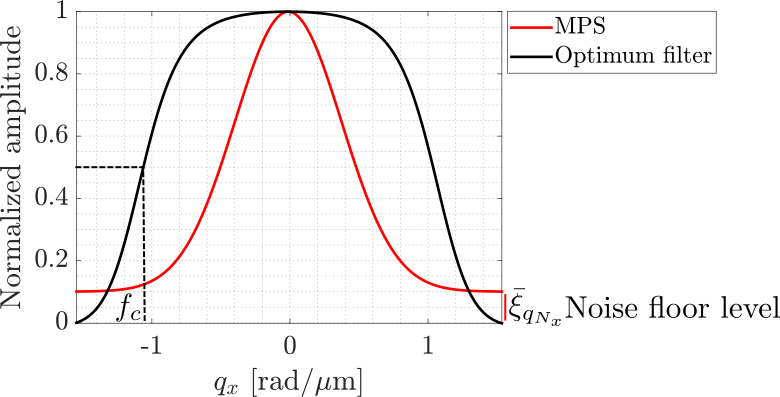
\includegraphics[width=.7\textwidth]{Figures/SHARP/OptimumFilterExample.pdf}
	\caption[Example of the optimum filter for a Gaussian MPS.]{Example of the optimum filter for a Gaussian MPS. $fc$: cutoff frequency of the filter.}
	\label{fig:OptimumFilter}
\end{figure}

Now that the phase stabilization and aberration correction procedures have been defined, the two 1D steps of SHARP can be condensed as
\begin{align}
    \tilde{S}^{\text{1D}}(x,y,z) &= \mathbb{A}_x\left\{ \mathbb{C}_x\left\{ S(x,y,z) \right\} \right\}, \\
    \tilde{S}(x,y,z) &= \mathbb{A}_y\left\{ \mathbb{C}_y\left\{ \mathbb{C}^{-1}_x\left\{  \tilde{S}^{\text{1D}}(x,y,z) \right\} \right\} \right\},
\end{align}
where $\tilde{S}^{\text{1D}}(x,y,z)$ is the partially corrected tomogram and $\tilde{S}(x,y,z)$ is the $x$-$y$-separable aberrations corrected tomogram.

There are some particularities to discuss in regard to the described procedure. First, the $x$-$y$ separability requirement has a direct limitation of the aberrations that can be corrected because not all aberrations can be separated into two 1D operations, only those whose deconvolution kernel can be separated into two 1D kernels. Among the $x$-$y$-separable aberrations, the most important for practical terms are defocus, $xy$-astigmatism, spherical aberration and $xy$-comma, being defocus the most relevant in many OCT applications given that it is intrinsic to the nature of the focused Gaussian beam used to illuminate the sample. In fact, defocus can be considered the only significant aberrations in many medical applications of OCT apart from retinal imaging where complex wavefronts may be induced by the eye of the subject. This means that SHARP is sufficient for many scenarios despite its $x$-$y$-separability requirement, in particular to numerically extend the depth of field (DoF), relaxing the DoF-lateral resolution--trade-off.

Another important aspect is in regard to the role of the roll-back step. The process of phase noise correction along the first axis adds random phase errors along the orthogonal axis that can become strong enough to frustrate the subsequent phase correction along the second axis, resulting in a lower local phase stability than the case of correcting the second axis directly, i.e. without correcting the first axis previously. The purpose of the RB step is thus to cancel out the first phase noise correction in order to avoid any phase noise induced in the first correction. It can be noted that the RB step uses the phase noise correction computed before correcting aberrations along first axis but the RB is performed after correcting aberrations that may change the phase pattern. Interestingly, the aberration correction applied along the first axis does not perturb the relative phase relation in the second axis although the phase pattern itself may have changed, hence the exact same phase noise correction is still valid for the RB (but conjugated) even though it is applied after aberration correction.

\section{Proof of concept experimental validation}\label{sec:Test}

\section{Extending SHARP}\label{sec:Extensions}

\subsection{Complex amplitude motion artifacts correction}

Relevant effects of motion in the OCT signal for the context of CAC were already explain in Section.~\ref{sec:phaseStab}, namely complex-amplitude shift and phase-jump. The latter often has a greater relevance for CAC, thus phase noise correction methods commonly address phase offsets, including the phase stabilization performed in SHARP. However, in many \text{in vivo} applications, complex-amplitude shift may also have a significant influence and could even be more noticeable since they affect both the phase and the amplitude of the tomogram, appearing as signal distortions in the structural image.

Motion artifacts can be avoided using fast systems with volume acquisition rate such that sample appears static during the scanning, for instance recent reports have achieved volume acquisition rates in the order of tents of milliseconds~\cite{Auksorius2020_vivo}, but employing very specialized components. With A-line acquisition rates of the order of 100~kHz in current widespread systems, it is possible to assume that, in normal conditions, the sample is static during the acquisition of a single B-scan and motion manifests as rigid-body displacements across different B-scans, in other words, as intra-B-scan bulk motion. In such case, complex-amplitude shifts can be corrected straightforwardly using sub-pixel image registration.

The idea of bulk image registration is to find the relative global shift between two given images $I_1(m,l)$ and $I_2(m,l)$. Most used method is intensity-based registration where the cross-correlation $r_{\text{cc}} = I_1(m,l)\star I_2(m,l)$ of the two images is computed and the location of the peak is found to determined the relative shift $(m_{\text{cc}}, l_{\text{cc}})$ between the two images, Then, the shift is applied to one of the two images in order to match this to the other. Commonly, cross-correlation is computed in Fourier domain as 
\begin{equation}\label{eq:ImageReg}
    r_{\text{cc}} = \text{FT}^{-1}_{q_m,q_l}\left\{\text{FT}_{m,l}\left\{I_1(m,l)\right\}\text{FT}_{m,l}\left\{I_2(m,l)\right\}\right\}
\end{equation}
and the shift is corrected as
\begin{equation}
    I_2 = \text{FT}^{-1}_{q_m,q_l}\left\{\text{FT}_{m,l}\left\{I_2(m,l)\right\} \exp\left[-i2\pi\left(m_{\text{cc}} \frac{q_m}{M} + l_{\text{cc}} \frac{q_l}{L}\right)\right]\right\}
\end{equation}
where $m_{\text{cc}}$ and $l_{\text{cc}}$ are given in pixels and $M$ and $L$ are the image sizes.

When a sub-pixel estimation is required, the product of the two Fourier-transformed images in Eq.~\eqref{eq:ImageReg} is zero-padded prior to computation of the inverse FT in order to have an upsampled cross-correlation $r_{\text{cc}}$. However, this zero-padding will increase the size of the input of the inverse FT increasing computational cost significantly specially when a high sub-pixel resolution is required, for instance of $1/20$ requiring a zero-padding of $20M\times 20L$. Fortunately, there are efficient sub-pixel image registration methods that significantly improve speed without sacrificing accuracy~\ref{}.

Using efficient sub-pixel image registration, it is possible to include a step for intra-B-scan bulk motion correction in SHARP procedure. This step, if necessary, is performed after the first phase stabilization step since registering the complex signal requires phase stable data. Complex-shift correction would enable operation of subsequent steps of SHARP for \textit{in vivo} imaging. Motion correction is performed by registering adjacent B-scans $n$ and $n-1$ and finding the relative lateral and axial shifts $(m_\text{cc}(n), l_\text{cc}(n))$ as
\begin{equation}
    (m_\text{cc}(n), l_\text{cc}(n)) = \arg\left\{\max\left\{ S(m,n,l)\star S(m,n-1,l) \right\}\right\}
\end{equation}
where cross-correlation is performed inside the B-scan plane, i.e. along coordinates $x$ and $z$, Shifts across B-scans are accumulated to computed global shifts with respect to first Bscan,
\begin{equation}
    I_2 = \text{FT}^{-1}_{q_m,q_l}\left\{\text{FT}_{m,l}\left\{I_2(m,l)\right\} \exp\left[-i2\pi\left(m_{\text{cc}} \frac{q_m}{M} + l_{\text{cc}} \frac{q_l}{L}\right)\right]\right\}
\end{equation}

\subsection{Spatially-varying aberrations correction}

\subsection{Complex amplitude noise reduction}

\subsection{Correction of arbitrary aberrations}